\documentclass[main]{subfiles}

\begin{document}


\chapter{Verificaciones de los par\'ametros obtenidos}
\label{chap:verificaciones_modelado}

Una vez caracterizado el sistema en cuanto a las ecuaciones que lo gobiernan y los par\'ametros involucrados se busca validar dichos resultados por medios alternativos. Como puede observarse en las ecuaciones \ref{eq:modelo} se tiene un subsistema que es independiente del resto de las variables, el de los \'angulos de Euler y las velocidades angulares. Es fundamental que este sistema se encuentre bien caracterizado a fin de desarrollador un controlador adecuado para el mismo.\\ 

Si restringimos el movimiento del cuadric\'optero a un giro segu\'un la direcci\'on $\vec{x}_q$ las ecuaciones que gobiernan al sistema linealizado en torno a las condiciones $\psi = \omega_{qx} = 0$ y $\omega_1 = \omega_3 =\omega_{hovering}$ son:
\begin{equation}
\label{eq:mod_psi}
\left(\begin{array}{c}
\dot{\psi}\\
\dot{\omega}_{qx}
\end{array}\right) = \left(\begin{array}{cc}
0 & 1\\
-\frac{MgL^\prime}{I_{xx}} & 0
\end{array}\right)\left(\begin{array}{c}
\psi\\
\omega_{wx}
\end{array}\right) + b\left(\begin{array}{cc}
0 & 0\\
1 & -1
\end{array}\right)\left(\begin{array}{c}
\omega_2\\
\omega_4
\end{array}\right)
\end{equation}

Donde
\begin{equation}
b =L\frac{2b_1\omega_{hovering}+b_2}{I_{xx}}
\end{equation}

La transferencia del sistema entre el \'angulo $\psi$ y la diferencia $\omega_2-\omega_4 (\Delta \omega)$ tiene la forma:

\begin{equation}
\label{eq:trans_psi}
H_{\psi}(s) = \frac{b}{s^2+\frac{MgL^\prime}{I_{xx}}}
\end{equation}

Analizando la respuesta al escal\'on de dicho \'angulo podemos obtener algunas relaciones que sirven para verificar las caracterizaciones realizadas. Inicialmente se tiene $\Delta \omega_i = -22.4 rad s^{-1}$, se aplica un escal\'on tal que $\Delta \omega_f = 13.5 rad s^{-1}$. En la figura \ref{fig:esc_psi} puede observarse la respusta del \'angulo $\psi$ a dicho escal\'on. En primer lugar cabe aclarar que el escal\'on se comporta acorde al modelo realizado ya que si as\'i fuese la oscilaci\'on no deber\'ia extinguirse, el decaimiento de la oscilaci\'on se debe a efectos no considerados en el set-up experimental, como por ejemplo la fricci\'on.\\

\begin{figure}
  \centering
 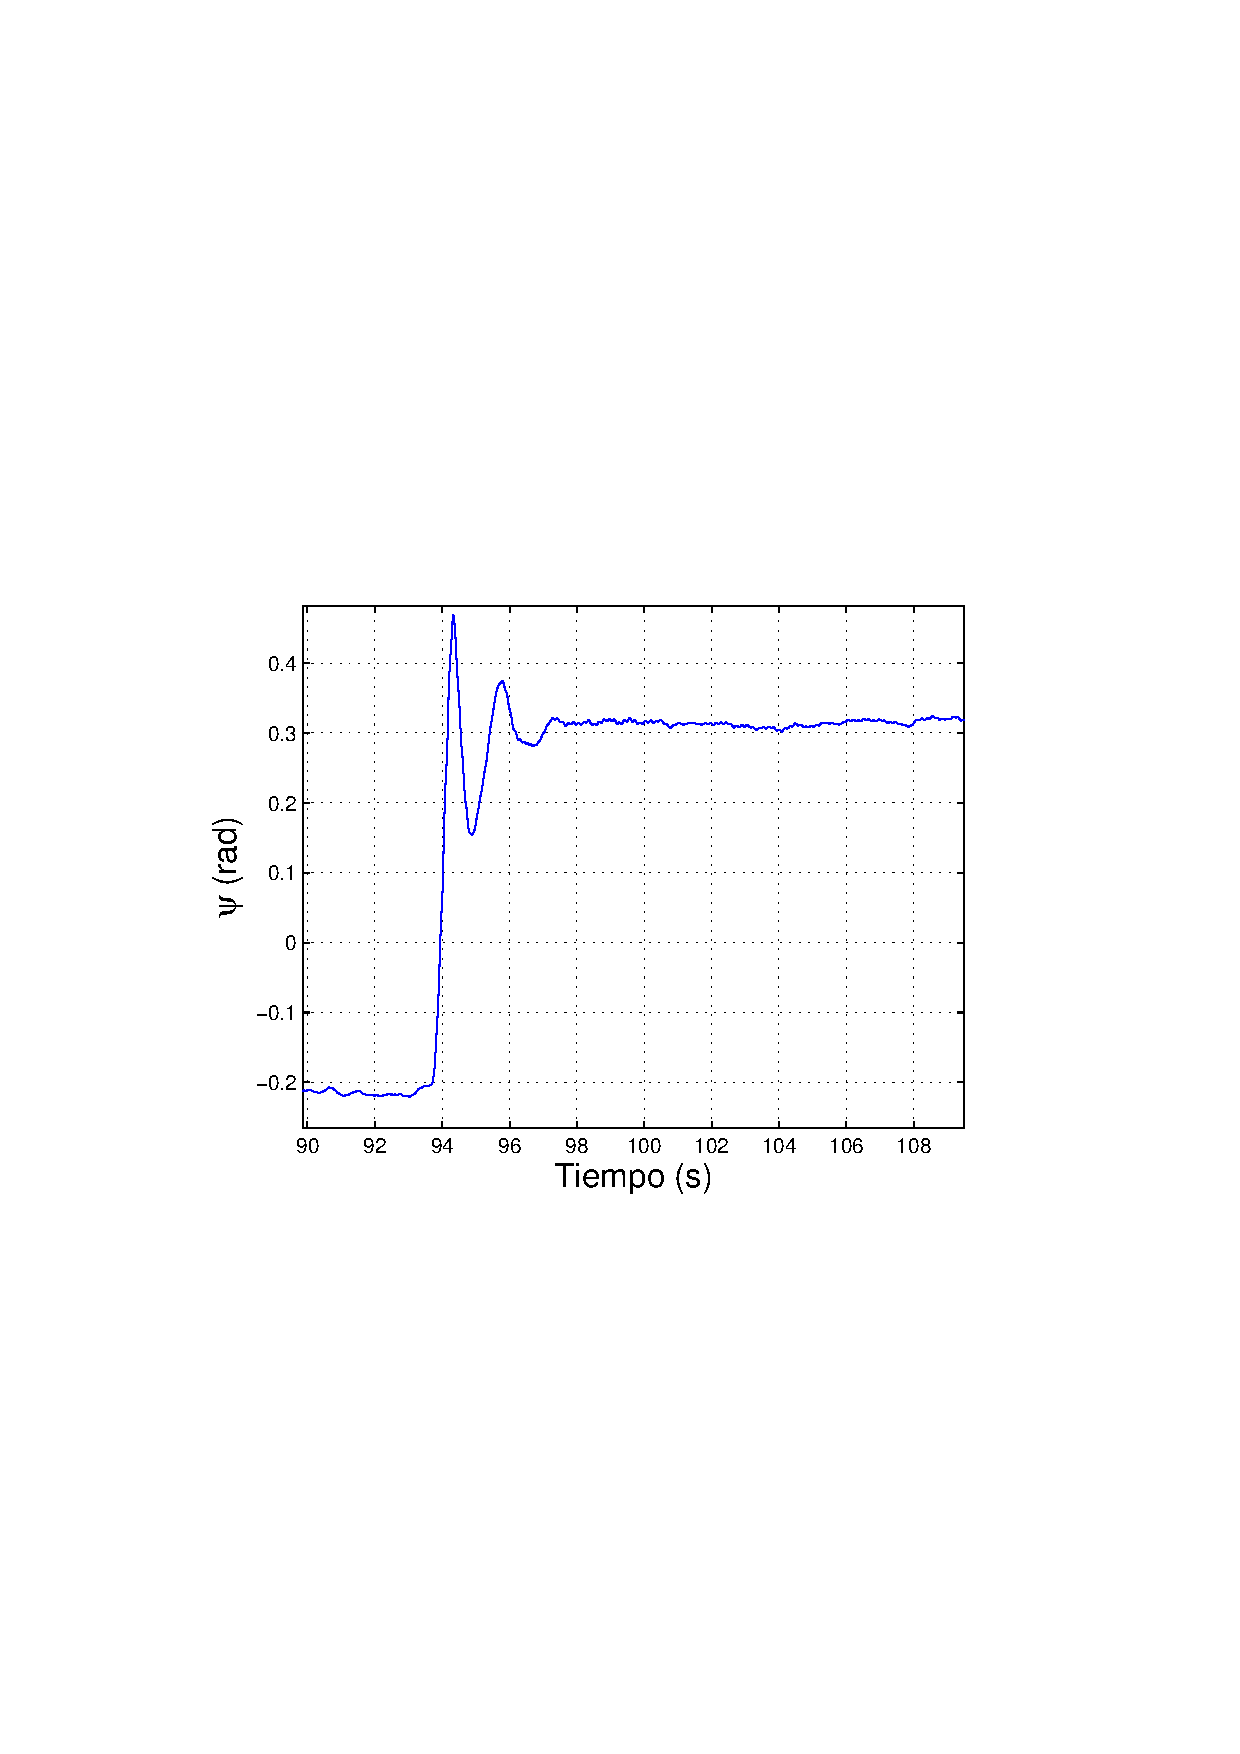
\includegraphics[width=0.8\textwidth]{./pics_verificacion/esc_psi}
  \caption{Respuesta al escal\'on del \'angulo $\psi$}
  \label{fig:esc_psi}
\end{figure}

De acuerdo a la figura \ref{fig:esc_psi} al aplicar un escal\'on en la entrada de $\Delta \omega_f - \Delta \omega_i = 35.9 rad s^{-1}$ el \'angulo $\psi$ varia desde $-0.22 rad$ alcanzando un valor en r\'egimen de $0.33 rad$, la variaci\'on total de dicho \'angulo es de $0.55 rad$. Por lo tanto la ganancia de la transferencia \ref{eq:trans_psi} es $\frac{0.55}{35.9}  \approx 0.015 s$. La ganancia de la transferencia puede expresarse adem\'as como $H_{\psi}(0)$. Por lo tanto se tiene que:

\begin{equation}
\frac{bI_{xx}}{MgL^\prime} = 0.015 s
\end{equation}

Por otra parte, si bien la respuesta al escal\'on experimental no se corresponde perfectamente con el modelo te\'orico, puede aproximarse el per\'iodo de las oscilaciones en el transitorio por el per\'iodo te\'orico $T_teo = \frac{2\pi}{\omega}$ donde $\omega = \sqrt{\frac{MgL\prime}{Ixx}}$. Bajo estas suposiciones el per\'iodo de acuerdo a la respuesta al escal\'on experimental es $1.2s$. Obtenemos entonces:

\begin{equation}
\omega = \frac{2\pi}{T} = \sqrt{\frac{MgL^\prime}{I_{xx}}}=5.23 s
\end{equation}

Si bien no es posible determinar absolutamente todos los par\'ametros del sistema si podemos calcular $b$ utilizando que:

\begin{equation}
b = H(0)\omega^2 = 0.41 s^{-1}
\end{equation}

Los valores calculados a partir de los par\'ametros determinados experimentalmente son:
\begin{itemize}
	\item $b = 0.35 s^{-1}$
	\item $\omega = \sqrt{\frac{MgL^\prime}{Ixx}} = 6.5s$
\end{itemize}

Los errores relativos entre los valores te\'oricos y experimentales para los par\'ametros $b$ y $\omega$ son del $14.6\%$ y del $24.32\%$ respectivamente. Estos errores no son para nada despreciables y pueden introducir diferencias significativas en el comportamiento del sistema en lazo cerrado simulado y el real.\\

  


\end{document}